\documentclass [a4paper, 11pt] {article}

%document configuration
\newcommand{\courseName}{Machine Learning in Graphics \& Vision}
\newcommand{\termYear}{Summer Term 2020}
\newcommand{\homeworkNum}{4}
\newcommand{\studentOne}{Driton Goxhufi}
\newcommand{\studentTwo} {Damir Ravlija}
\newcommand{\matrikelNrStOne}{4233242}
\newcommand{\matrikelNrStTwo}{5503184}
\newcommand{\mailStOne}{driton.goxhufi@student.uni-tuebingen.de}
\newcommand{\mailStTwo}{damir.ravlija@student.uni-tuebingen.de}

%packages
\usepackage [english] {babel}
\usepackage [T1] {fontenc}
\usepackage [utf8] {inputenc}
\usepackage {graphicx}
\usepackage {subcaption}
\usepackage {amsmath}
\usepackage {amssymb}
\usepackage {amstext}
\usepackage {amsthm}
\usepackage {listings}
\usepackage {tikz}
\usepackage[
pdftex,
pdfauthor={Goxhufi, Driton; Ravlija, Damir},
pdftitle={MLGV - Exercise \homeworkNum Submission},
pdfsubject={Machine Learning in Graphics \& Vision Homework}
]{hyperref}

\usepackage[a4paper,lmargin={2cm},rmargin={2cm},tmargin={3.5cm},bmargin = {2.5cm},headheight = {4cm}]{geometry}

\usepackage[shortlabels]{enumitem}
\usepackage{lastpage}
\usepackage{fancyhdr}

\usepackage{lipsum}
\usepackage{ifthen}

\pagestyle{fancy}



%other config
\renewcommand{\v}[1]{\boldsymbol{#1}}
\newcommand{\mat}[1]{\boldsymbol{#1}}
\newcommand{\m}[1]{\begin{pmatrix}#1\end{pmatrix}}
\newcommand{\tr}[2]{{}^{#1}T_{#2}}
\graphicspath{{./images/}}


\lhead{\begin{tabular}{l}
		\courseName\\
		\termYear \\
		Exercise \homeworkNum
\end{tabular}}
\rhead{\begin{tabular}{lr}
		\studentOne & \matrikelNrStOne \\
		\studentTwo & \matrikelNrStTwo \\
\end{tabular}}

\begin{document}
	
\title{\vspace{-1.5cm}\textbf{Exercise \homeworkNum} \\ 
	\courseName}
\author{\begin{tabular}{lcr}
		\studentOne & \matrikelNrStOne & \href{mailto:\mailStOne}{\mailStOne} \\
		\studentTwo & \matrikelNrStTwo & \href{mailto:\mailStTwo}{\mailStTwo} 
\end{tabular}}	
\date{}
\maketitle


\section*{Task 1}
\begin{enumerate}
\item[(c)]
It seems that using the window size 3 leads to better visual results because although window size 3 produces a lot of artifacts and the image is noisy, it has more details than the images produced by larger window sizes which suffer from loss of details as parts become too smooth.

\item[(d)]
We think that block matching approach fails to lead to good estimations around homogeneous regions because since these regions have mostly the same color values, multiple window blocks in these regions have similar sums of absolute difference (SAD) values.


\end{enumerate}

\section*{Task 2}
\begin{enumerate}
\item[(c)]
When the initial parameters with 64 filter numbers and 1000 iterations were used, loss did not decrease significantly, but a certain downward trend was visible (Figure \ref{fig:64-1000}). The best training loss and accuracy that we got after training 1000 iterations was:
\begin{lstlisting}
Loss:0.1965 	Accuracy: 0.557
\end{lstlisting}

\begin{figure}[!h]
	\centering
	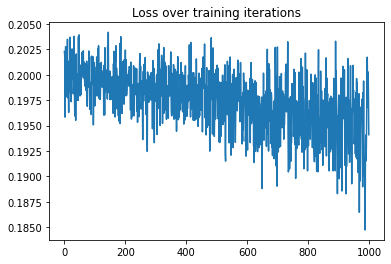
\includegraphics[width=0.8\textwidth]{img/64-1000.png}
	\caption{Task 2.c) Training loss over iterations when training with filter number 64 and 1000 iterations.}
	\label{fig:64-1000}
\end{figure}

When we increased the number of iterations to 5000 the model continued improving (Figure \ref{fig:64-5000}) and the best loss and accuracy achieved was:
\begin{lstlisting}
Loss:0.1238 	Accuracy: 0.746
\end{lstlisting}
\begin{figure}[!h]
	\centering
	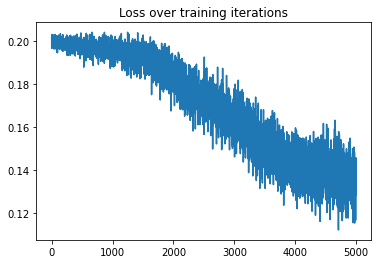
\includegraphics[width=0.8\textwidth]{img/64-5000.png}
	\caption{Task 2.c) Training loss over iterations when training with filter number 64 and 5000 iterations.}
	\label{fig:64-5000}
\end{figure}

When the number of filters was decreased to 32, the loss did not significantly decrease with the increased number of iterations (Figure \ref{fig:32-128}). On the other hand, increasing the filter number to 128 did not result in significantly improved results compared to using filter number 64.

From our findings it seems that the increased number of iterations is advantageous only with the increasing filter number since the smaller network with filter number of 32 could not significantly improve in 5000 iterations. Furthermore, since the networks with filter numbers 64 and 128 improve even after more than 5000 iterations, it seems that 1000 iterations is not enough to train the model, while the decreased loss and improved accuracy that are achieved with larger filter numbers become visible only if they are accompanied by increased number of iterations (Figure \ref{fig:32-128}).

\begin{figure}[!h]
	\centering
	\begin{subfigure}{0.4\textwidth}
		\centering
		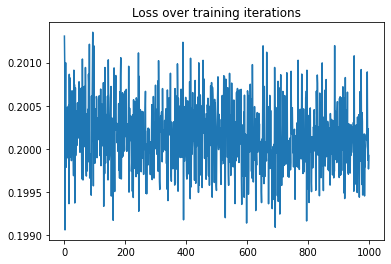
\includegraphics[width=\textwidth]{img/32-1000.png}
		\caption{Filter number 32, Iterations 1000}
		\label{fig:32-1000}
	\end{subfigure}
	\begin{subfigure}{0.4\textwidth}
		\centering
		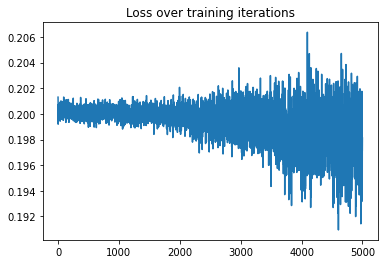
\includegraphics[width=\textwidth]{img/32-5000.png}
		\caption{Filter number 32, Iterations 5000}
		\label{fig:32-5000}
	\end{subfigure}
	\begin{subfigure}{0.4\textwidth}
		\centering
		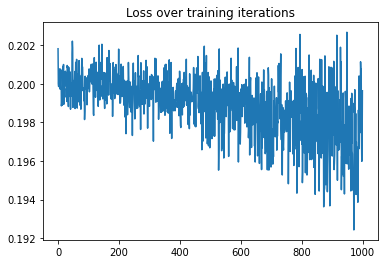
\includegraphics[width=\textwidth]{img/128-1000.png}
		\caption{Filter numbers 128, Iterations 1000}
		\label{fig:128-1000}
	\end{subfigure}
	\begin{subfigure}{0.4\textwidth}
		\centering
		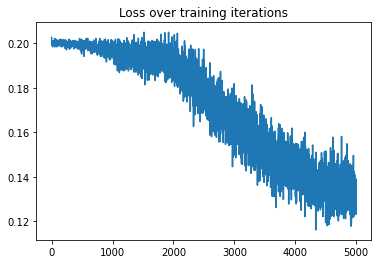
\includegraphics[width=\textwidth]{img/128-5000.png}
		\caption{Filter number 128, Iterations 5000}
		\label{fig:128-5000}
	\end{subfigure}
	\begin{subfigure}{0.4\textwidth}
		\centering
		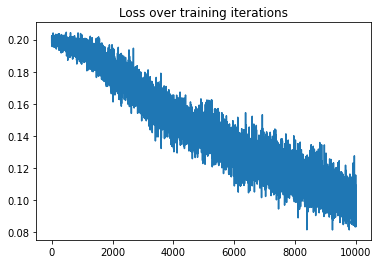
\includegraphics[width=\textwidth]{img/64-10000.png}
		\caption{Filter numbers 64, Iterations 10000}
		\label{fig:64-10000}
	\end{subfigure}
	\begin{subfigure}{0.4\textwidth}
		\centering
		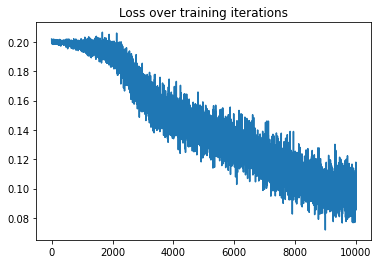
\includegraphics[width=\textwidth]{img/128-10000.png}
		\caption{Filter number 128, Iterations 10000}
		\label{fig:128-10000}
	\end{subfigure}
	\caption{Task 2.c) Training loss over iterations.}
	\label{fig:32-128}
\end{figure}

\item[(d)]
Predictions by the Siamese Neural Network seem to be better than the ones obtained by the block matching algorithm because although the visualization is much smoother than block matching with window size 3, it doesn't suffer from as much detail loss as visualization obtained using block matching with larger window sizes. Difference in the predictions is the most dominant in the texture-less road region near the camera.

\end{enumerate}


\end{document}

